\section{Architecture Overview}

In this chapter, we will review the architectures of Multi-access Edge Computing and the enabling key technologies like Network Functions Virtualization.

\subsection{Introduction to Multi-access Edge Computing}

\begin{figure}
	\centering
	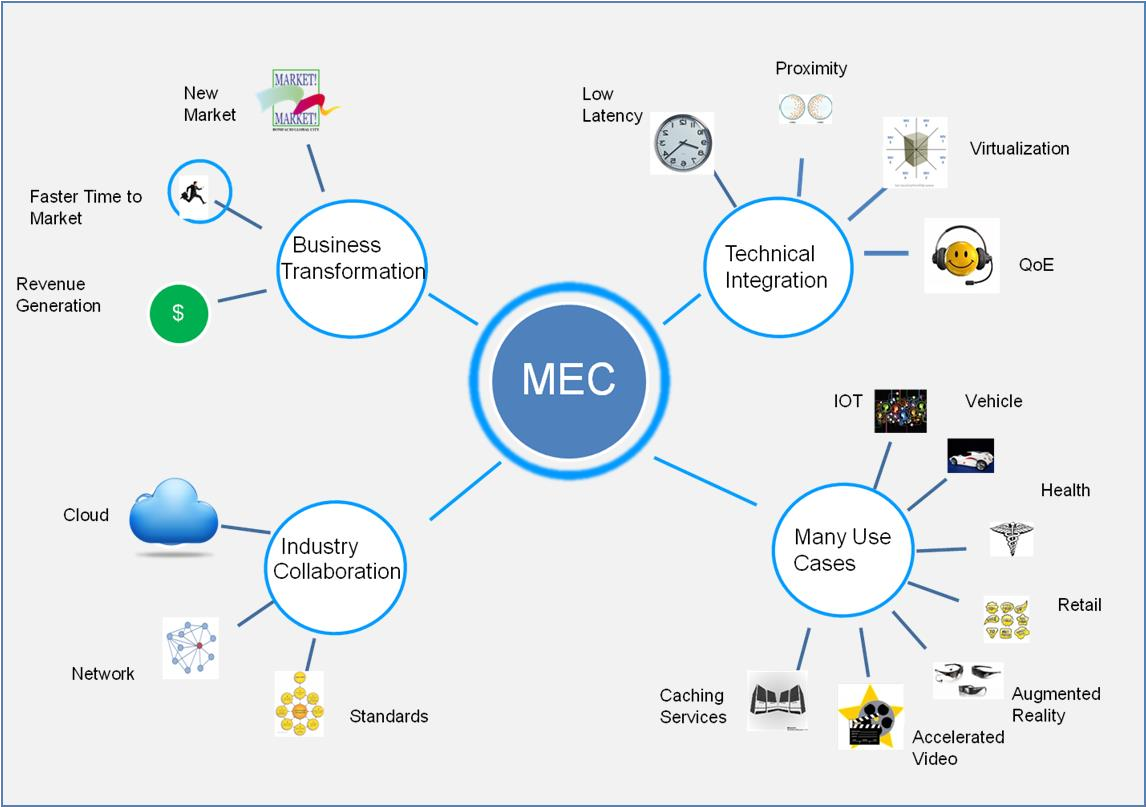
\includegraphics[width=0.9\textwidth]{mec_market_drivers}
	\label{fig:figure3}
	\caption{MEC Market Drivers}
\end{figure}

Edge Computing refers to carrying out complete or part of the computation at the edge device instead of moving the data to the data center or cloud. There are obvious advantages to this methodology. The key advantage being effective bandwidth utilization due to proximity of data sources to the computation center. It also allows for new kind of services that reside on the edge giving rise to applications in the area of health care, automotive, industrial automation and mobile gaming along with the new and upgraded telecommunication services. 

While MEC emerged as a key enabler for 5G technology, it has broad applications in 4G deployments as well and when paired with other technologies like Cloud RAN, NFV, IOT, a whole new horizon of new service possibilities emerges. 
